We first describe the multi-agent surveillance synthesis problem informally, in the context of a motivating case study. 

We consider wildlife conservation in Africa, in particular, at the Selous Game Reserve (SGR) located in Tanzania, where the African Black Rhinoceros population is under serious threat due to poaching. We are motivated by a recommended anti-poaching initiative in the SGR by the World Heritage Centre,  to study the use of a sensor network for tracking the position of a potential poacher  with user-specified precision. Since the SGR is a very large area, the network consists of both mobile and static sensors. We apply the  distributed synthesis method proposed in this paper to synthesize surveillance strategies for the mobile sensors that satisfy the desired tracking requirement.


\begin{figure}
\centering
\subfloat[SGR interior landscape \cite{UN13} \label{fig:SGR-map}]{
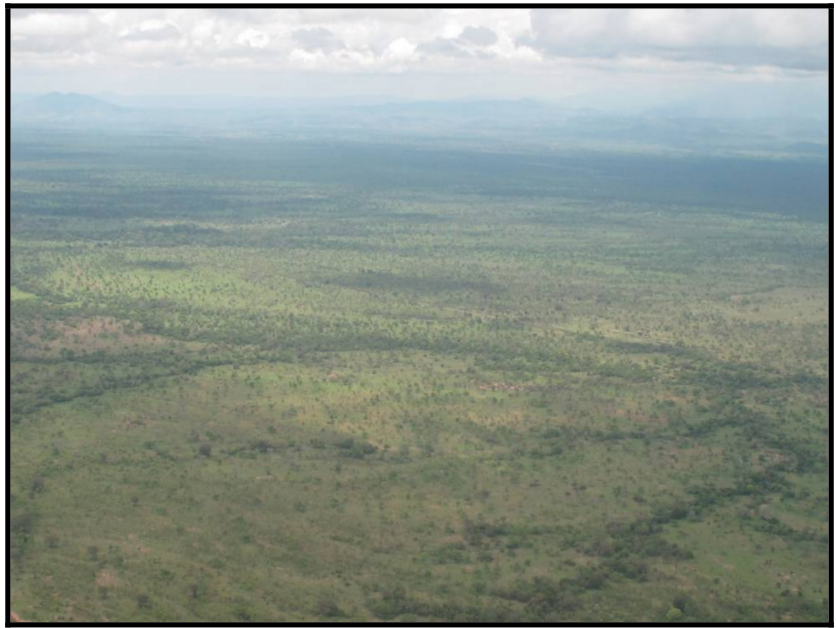
\includegraphics[scale=0.15]{figs/SGR.png}
}\hspace{1cm}
%\hfill
\subfloat[Grid representation of the landscape in \ref{fig:SGR-map} \label{fig:SGR-grid}]{
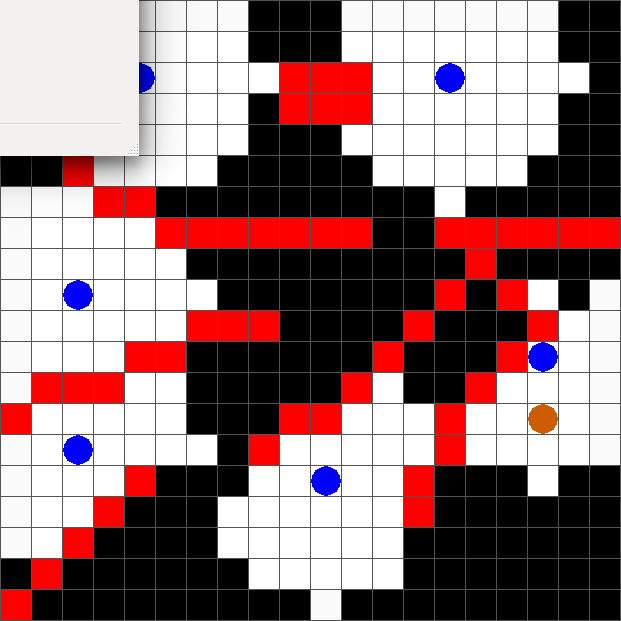
\includegraphics[scale=0.15]{figs/SGR-grid-vis.png}
}

\caption{The landscape in \ref{fig:SGR-map} is coarsely represented as the gridworld in \ref{fig:SGR-grid}. The red regions represent impassable terrain. The yellow areas are the ones covered  by static sensors.}\vspace{-0.5cm}
\label{fig:casestudy}
\end{figure}

Figure \ref{fig:casestudy} shows a section of the SGR that we represent as a gridworld which will form the state space of the game. Each static sensor monitors a given area of the grid (shown in yellow) and detects any presence of the target (i.e., threat) in these states, but cannot determine the target's exact location. The  requirement is to ensure that over and over again, the set of potential locations of the target is reduced to $5$ cells. In other words, every time the target escapes from the vision of all  sensors, the network guarantees that eventually the uncertainty about its position will be reduced to $5$ grid cells.


